%11/10 - Luis del Peso
\chapter{Alineamiento de múltiples secuencias (MSA)}
¿Cuál es la ventaja del MSA frente a los alineamientos por pares? La principal ventaja es que hay mucha más información en un MSA que en un alineamiento por pares, por lo que al realizar un MSA mejoramos la relación señal/ruido. Consideremos el ejemplo de juguete de la figura \ref{fig:msa}. Muestra la alineación de un fragmento del dominio Ser/Thr-quinasa del AK77 humano con dos proteínas de archaea. Ambas alineaciones por pares son relativamente similares, por lo que sería difícil decidir cuál de ellas, si es que hay alguna, representa un verdadero homólogo de la consulta (los valores E son $3 \cdot 10^6$ y $7 \cdots 10^7$ respectivamente). Además, incluso sabiendo que el segundo alineamiento corresponde a un verdadero homólogo, sería difícil identificar qué residuos son esenciales para la actividad y/o el plegamiento del dominio quinasa. Sin embargo, un MSA de miembros de la familia Ser/Thr-quinasa revela los residuos clave del dominio catalítico. Además, esta información indica que el primer alineamiento corresponde a un falso positivo. Esto significa que, a pesar del valor E relativamente bajo, es poco probable que las proteínas alineadas compartieran un ancestro común. Este ejemplo también muestra que el MSA de un grupo de secuencias homólogas define los dominios o motivos que caracterizan a una familia de proteínas. Los residuos alineados en un MSA se derivan presumiblemente de un ancestro común, es decir, son homólogos en un sentido evolutivo. En consecuencia, los residuos conservados en un MSA tienden a ocupar posiciones correspondientes en la estructura tridimensional de cada una de las proteínas homólogas. Es importante señalar que las estructuras tienden a estar más conservadas que las secuencias dentro de una familia de proteínas. Así, para dos proteínas homólogas distantes, la conservación a nivel de residuos podría ser baja, por ejemplo un 30\% de identidad, mientras que tienen una proporción mucho mayor de residuos, por ejemplo un 50\%, localizados en posiciones equivalentes de sus estructuras tridimensionales. En consecuencia, los verdaderos homólogos distantes suelen tener una función bioquímica/biológica similar a pesar de la baja identidad de secuencia. Y lo que es más importante, utilizando MSA podríamos alinear dos secuencias distantes a través de su relación con una tercera secuencia, integrando así información no disponible en alineaciones por pares. Por ejemplo, si las proteínas A y C son homólogas muy distantes, un MSA que incluya una proteína B, relacionada tanto con A como con C, podría ayudar a construir el alineamiento correcto si B es equidistante a A y B en distancia evolutiva.

\begin{figure}[htbp]
\centering
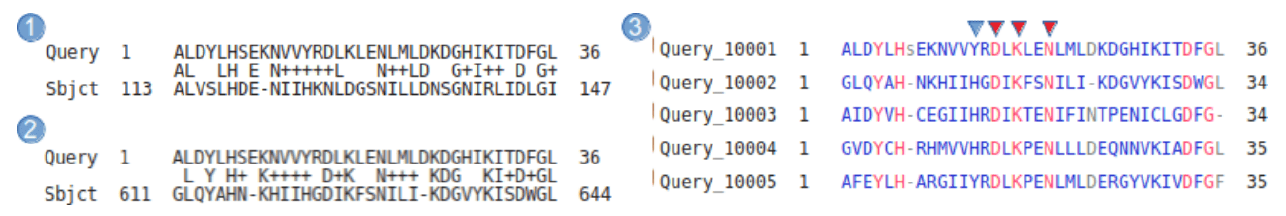
\includegraphics[width = \textwidth]{figs/msa.png}
\caption{\textbf{Pairwise vs MSA}. Se utilizó un fragmento del dominio quinasa de AKT7 humano (P31749) como consulta para buscar en una base de datos de proteínas archaca. (1) Alineación de AKTI y una ATPasa de la familia AAA (WP\_109940497.1) de \textit{Methanospirillum stamsii}. (2) Alineamiento del mismo fragmento de AKTI con una serina/treonina-proteína quinasa (OPY23844) de \textit{Methanobacterium sp}.. (3) MSA del sitio activo de 5 serina-treonina quinasas distantes. En flecha roja los residuos conservados en las 5 secuencias alineadas. Las puntas de flecha rojas marcan tres posiciones invariantes conservadas en todas las Ser/Thr-cinasas conocidas, el residuo Asp (D en esta tríada es el residuo del sitio activo. La punta de flecha azul marca una posición que está ocupada por His o Tyr en todas las proteínas conocidas de esta superfamilia).}
\label{fig:msa}
\end{figure}

\section{Métodos y esquemas de puntuación para la alineación de secuencias múltiples}
Como se explica en el capítulo anterior, la alineación óptima por pares puede lograrse eficazmente mediante algoritmos de programación dinámica. Estos métodos se basan en la construcción de una matriz $n \cdot m$, donde n y m corresponden a la longitud de las secuencias alineadas, y su complejidad en tiempo de ejecución es del orden de $O(n \cdot m)$ u $O(n^2)$ suponiendo que $n \sim m$. La extensión de este método a MSA es trivial. Por ejemplo, para tres secuencias de longitudes n, m y k, construiríamos una matriz $n \cdot m \cdot k$ que contenga las puntuaciones parciales óptimas para el alineamiento de tres posiciones. Sin embargo, la complejidad temporal en este caso sería de $O(n \cdot m \cdot k)$ u $O(n^3)$ suponiendo que $n \sim m \sim k$. De forma más general, para s secuencias de longitud n, la complejidad temporal sería $O(n^s)$ que crece exponencialmente con el número de secuencias. Por lo tanto, aunque este enfoque conduciría a un MSA óptimo, es poco práctico para más de unas pocas secuencias. Por este motivo, los métodos «simultáneos» no pueden aplicarse a problemas reales de MSA y se aproximan mediante métodos heurísticos que reducen el tiempo de cálculo pero no garantizan encontrar el alineamiento múltiple óptimo. Uno de los programas más populares para realizar MSA es ClustalW. Es un ejemplo de una familia de algoritmos que siguen una estrategia progresiva o jerárquica. Los métodos progresivos funcionan en tres pasos (véase la figura \ref{fig:clustalw}):
\begin{enumerate}
\item En el primer paso, este programa computa todos los posibles alineamientos por pares y calcula una puntuación bruta para cada alineamiento. La puntuación puede ser simplemente el porcentaje de identidades o medidas más sofisticadas.
\item A continuación, se realiza un análisis jerárquico de conglomerados en la tabla de puntuaciones por pares del paso anterior. Esta técnica produce un árbol guía o dendrograma que agrupa las secuencias según su similitud.
\item Por último, las secuencias se alinean progresivamente siguiendo la topología del árbol generado en el paso anterior. Así, se alinean las dos secuencias con la puntuación de similitud más alta y, a continuación, la secuencia siguiente se añade al alineamiento por pares o se utiliza en otro alineamiento por pares. Aunque no entraremos en detalles aquí, existen métodos rigurosos para alinear una secuencia contra un alineamiento. Imaginemos que la secuencia se alinea con una secuencia consenso derivada del alineamiento. El MSA puede representarse mediante estructuras matemáticas denominadas perfiles. En algún momento, los perfiles se alinean con los perfiles. Por último, el MSA se genera siguiendo el árbol guía desde los nodos más terminales hasta la raíz.
\end{enumerate}

\begin{figure}[htbp]
\centering
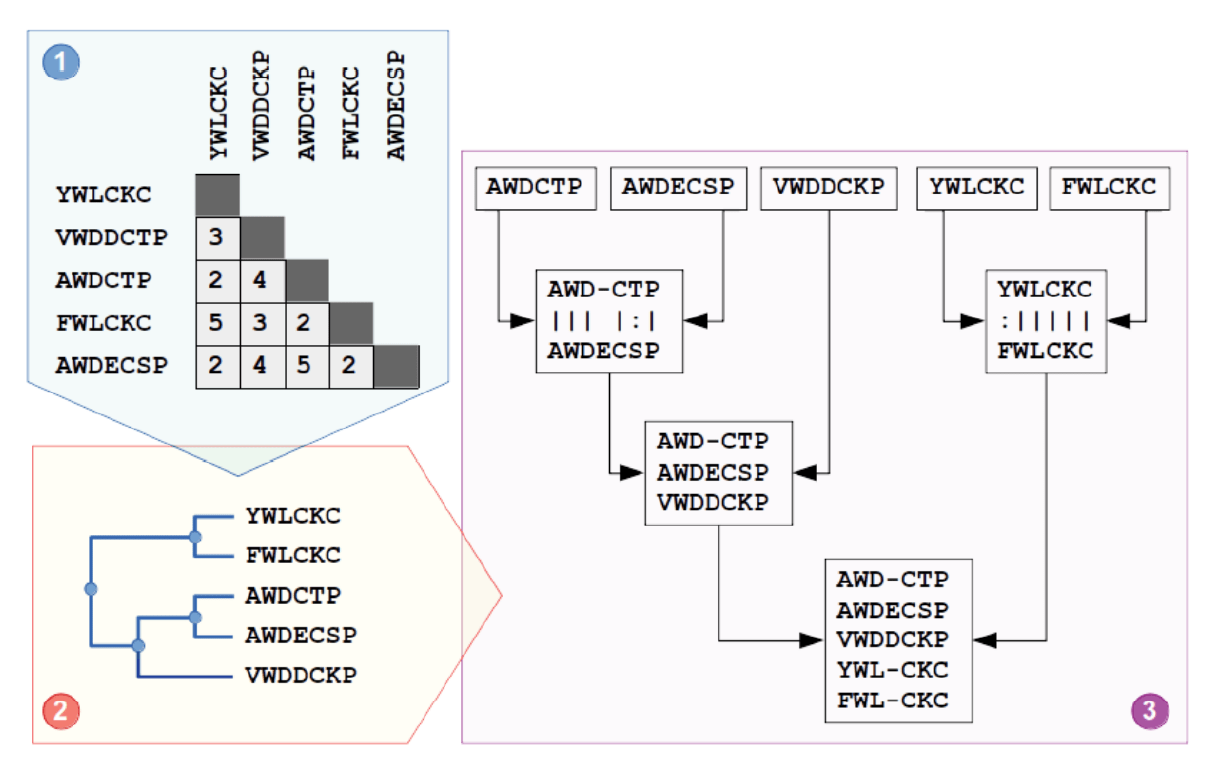
\includegraphics[width = \textwidth]{figs/clustalw.png}
\caption{\textbf{Métodos progresivos para el MSA}. Para producir un MSA de las secuencias YWLCKC (secuencia A), VWDDCTP (secuencia B). AWDCTP (secuencia C), FWLCKC (secuencia D) y AWDECSP (secuencia E), los métodos progresivos comparan primero todos los pares de secuencias (no mostrados) y registran la puntuación de cada alineamiento por pares (1). A continuación, basándose en estas puntuaciones, el algoritmo produce un árbol guía (2). Por último, las secuencias se alinean progresivamente empezando por las más cercanas. En cada paso del proceso, el algoritmo sigue la topología del árbol desde las hojas hasta la raíz, añadiendo nuevas secuencias o alineaciones en cada nodo del árbol (3).}
\label{fig:clustalw}
\end{figure}

Además de ClustalW, otras herramientas implementan variaciones de este algoritmo progresivo. Por ejemplo, ClustalW utiliza programación dinámica para el alineamiento por pares inicial, que es preciso pero puede ser lento para un gran número de secuencias. Por esta razón, otros métodos, como Kalign, cuentan el número de k-mers compartidos por las secuencias para calcular la distancia entre todos los pares. La ventaja de este método es que no es necesario alinear las secuencias para generar la matriz de distancias.

Uno de los problemas de los métodos progresivos es que el orden en que se añaden gradualmente las secuencias puede tener un fuerte impacto en el MSA final. Además, cuando se produce un error en un alineamiento intermedio, suele propagarse en los alineamientos posteriores. Esto es especialmente cierto en el caso de los gaps. Para mitigar estos problemas, diferentes algoritmos han adoptado variaciones en el procedimiento general, pero no las discutiremos aquí. Otro problema no resuelto en MSA es cómo calcular la puntuación. Se han propuesto varias estrategias:
\begin{itemize}
\item Scoring basado en una secuencia de referencia: $S_{MSA} = S_{AB} + S_{AC} + S_{AD} + S_{AE} $
\item Scoring basado en el dendograma: $S_{MSA} = S_{AB} + S_{CD} + S_{CD/E} + S_{AB/CDE}$
\item Scoring basado en la suma de alineamientos por pares: $S_{MSA} = S_{AB} + S_{AC} + S_{AD} + S_{AE} + S_{BC} + S_{BD} + S_{BE} + S_{CD} + S_{CE} + S_{DE}$
\end{itemize}

En resumen, aún no se ha resuelto el problema de calcular un MSA óptimo en un tiempo práctico. Mientras tanto, se han desarrollado varios enfoques heurísticos para calcular soluciones aproximadas que no garantizan ser la mejor solución posible.

Hasta ahora nos hemos centrado en el MSA de proteínas, sin embargo, el alineamiento múltiple de secuencias de regiones genómicas merece especial atención debido a la creciente cantidad de genomas completos disponibles y a su relevancia para identificar regiones genómicas reguladoras y comprender la variabilidad genética interindividual e interespecífica. Aunque no entraremos en detalles, la alineación de regiones genómicas plantea retos específicos. Por ejemplo, los genomas contienen un gran número de regiones repetitivas que son difíciles de alinear con precisión. Además, aunque la secuencia de determinadas regiones del genoma pueda conservarse en diferentes especies, a menudo la posición relativa de las distintas porciones del genoma no se conserva debido a reordenamientos genómicos. Por último, los MSA proteínicos suelen estar formados por un gran número de secuencias relativamente cortas, mientras que ocurre lo contrario con los MSA genómicos. Por todas estas razones, la alineación genómica requiere métodos de MSA especializados. Uno de ellos es MLAGAN, que se basa en un método progresivo similar al utilizado por ClustalW, y MULTIZ, utilizado para producir el MSA genómico que muestra el navegador del genoma de la UCSC.

\subsection{Ejemplo: FOXP2}
FOXP2 es un factor de transcripción. Al realizar un alineamiento de múltiples secuencias, se observan algunos residuos que presentan unos cambios únicos en humanos y son los que nos aportan la capacidad de comunicación como el habla. Además, individuos que tienen mutados esos individuos presentan un desorden del lenguaje. Por tanto, esos residuos son clave, y esto se demostró en ratones a los que se les cambió esos residuos concretos. Visto que esos cambios aparecen específicamente en humanos y que introducidos en ratones producen un comportamiento similar al habla, se analizó la filogenia y se observó exclusivamente en \textit{Homo sapiens} y Neandertales, pero no en otros primates.

\begin{figure}[htbp]
\centering
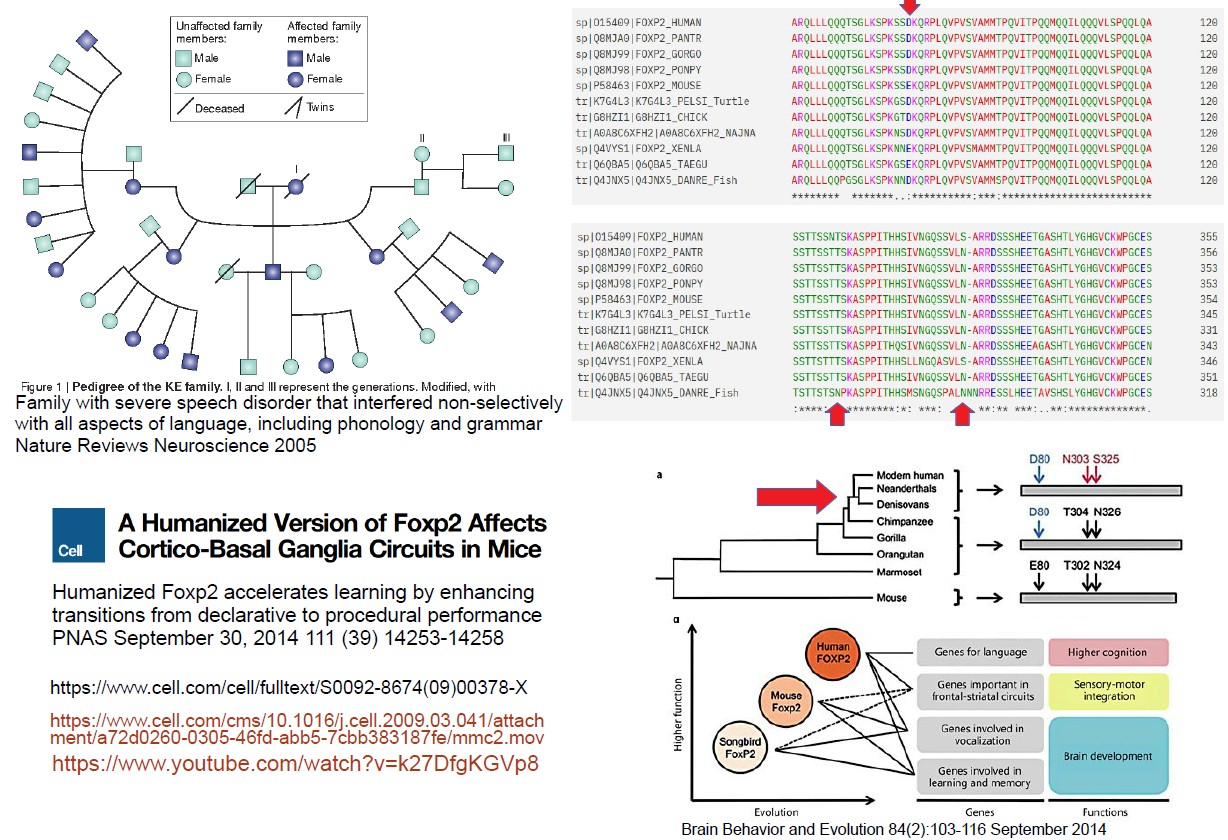
\includegraphics[width = \textwidth]{figs/foxp2.png}
\caption{Ejemplo del factor de transcripción FOXP2}
\end{figure}

%14/10 - Luis del Peso
\section{Representación de MSA}
Como se ha explicado anteriormente, el MSA puede utilizarse para identificar motivos/dominios funcionales y/o estructurales en un grupo de secuencias. Y lo que es más importante, una vez que hemos identificado ese motivo/dominio, puede utilizarse para buscar en bases de datos e identificar otras proteínas que compartan ese (nuevo) motivo y, como veremos, esas búsquedas son mucho más sensibles que las basadas en una secuencia de consulta. Sin embargo, para realizar dichas búsquedas, necesitamos una forma de representar el motivo/dominio revelado en el MSA. Existen varias formas de representar una región conservada, como se explica a continuación.

\subsection{Secuencia consenso}
Esta es la forma más sencilla de representar una región conservada y se utiliza ampliamente debido a su simplicidad y a su interpretación directa. Para construir una secuencia de consenso podríamos limitarnos a representar aquellos residuos que se conservan en todas las secuencias en una posición determinada. Por ejemplo, la secuencia consenso para la MSA representada en la figura \ref{fig:consensus-seq} es: TTxCxxAAxx donde x representa cualquier aminoácido. De hecho, esto se denomina consenso al 100\% de frecuencia, porque un residuo sólo se incluye en el consenso cuando está presente en el 100\% de las secuencias alineadas. El consenso puede construirse a cualquier otro nivel de porcentaje. Para el mismo alineamiento, el consenso al 50\%, que representa residuos presentes en al menos el 50\% de las secuencias, sería TTGCTCAAXT. Por último, a menudo el consenso representa el residuo más frecuente en cada posición, independientemente de su frecuencia absoluta.

\begin{figure}[htbp]
\centering
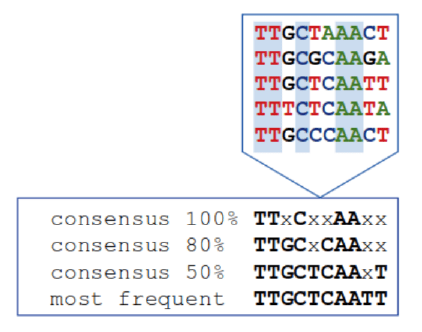
\includegraphics[width = 0.5\textwidth]{figs/consensus-seq.png}
\caption{\textbf{Secuencia consenso.} La secuencia de consenso indica el residuo presente en al menos un determinado porcentaje de las secuencias alineadas, o simplemente el residuo más frecuente, en cada posición del MSA. La figura muestra la alineación de varias secuencias de ADN unidas por C/EBP.}
\label{fig:consensus-seq}
\end{figure}

\subsection{Expresiones regulares o patrones}
El problema de las secuencias de consenso es que se pierde la mayor parte de la información contenida en el alineamiento. Por ejemplo, el consenso TTxCxxAAxx implica que no hay preferencia de residuo en la tercera posición. Sin embargo, la inspección de las secuencias individuales revela que, de hecho, existe una fuerte preferencia por la guanina en esta posición.
Por otra parte, el consenso del 50\% capta la preferencia por G en esta posición, pero no informa sobre qué otros residuos (si los hay) pueden ocupar esta posición ni sobre su frecuencia. Esta deficiencia es evidente en la décima posición del consenso del 50\%, que no muestra que en esta posición son posibles tanto la timina como la adenina. Las \textbf{expresiones regulares}, también conocidas como \textbf{patrones}, utilizan un conjunto de reglas para capturar esta diversidad. Por ejemplo, representan todos los residuos alternativos posibles en una posición determinada entre corchetes. También se puede representar aquellos residuos que nunca aparecen entre llaves. Así, el MSA de la figura \ref{fig:consensus-seq} puede representarse mediante la expresión regular:\\
TT[GT]C[TGC][AC]AA[TGC][TA]\\
TT[GT]C\{A\}[AC]AA\{A\}[TA]\\
Esta representación proporciona más información que las contras correspondientes, ya que muestra que la décima posición puede estar ocupada por T o A.

\subsection{Matrices de puntuación específicas para cada puesto (PSSM)}
Aunque las expresiones regulares representan una mejora con respecto al consenso, pierden importante información orientativa. La expresión regular mostrada en la sección anterior indica que T, C o G pueden encontrarse en las posiciones quinta y novena. Sin embargo, la preferencia por la timina es mayor en la quinta posición (0,6 frente a 0,4 de frecuencia). Una estructura que captura este tipo de información cuantitativa es la Matriz de Puntuación de Posiciones Específicas (PSSM). Una PSSM no es más que una matriz que confronta todos los símbolos posibles (los 20 aminoácidos posibles o los 4 nucleótidos en las secuencias de nucleótidos) con las posiciones de alineación. Cada celda de la matriz contiene un número que representa la preferencia de cada residuo concreto en cada posición. Hasta ahí, se consideraría una PWM (position weight matrix), es decir, tomar las frecuencias de cada nucleótido para cada posición normalizadas. Formalmente, los valores de cada celda de la PSSM se calculan como la relación logarítmica entre las frecuencias de residuos observadas en cada posición y las esperadas por azar. Así, suponiendo frecuencias de fondo iguales para todos los nucleótidos, el PSSM que representa el MSA mostrado en \ref{fig:consensus-seq} sería:

\begin{table}[htbp]
\centering
\begin{tabular}{l | l l l l l l l l l l }
& 1 & 2 & 3 & 4 & 5 & 6 & 7 & 8 & 9 & 10 \\ \hline
A & -1,2 & -1,2 & -1,2 & -1,2 & -1,2 & 0 & 1,4 & 1,4 & -1,2 & 0,4 \\
C & -1,2 & -1,2 & -1,2 & 1,4 & -0,2 & 1,2 & 1,2 & 1,2 & 0,4 & -1,2  \\
G & -1,2 & -1,2 & 1,2 & -1,2 & -0,2 & -1,2 & -1,2 & -1,2 & -0,2 & -1,2  \\
T & 1,4 & 1,4 & -0,2 & -1,2 & 0,8 & -1,2 & -1,2 & -1,2 & 0,4 & 0,8  \\
\end{tabular}
\caption{PSSM representando el MSA de la figura \ref{fig:consensus-seq}}
\end{table}

Por ejemplo, la entrada correspondiente a la timina en la posición 1 se calcularía como $log_2 \frac{5/5}{0,25} = 1,4$. Sin embargo, como $log_2(0)$ no está definido, esta ecuación produciría un error si se aplicara a la entrada de A en la primera posición $(log_2(\frac{0/5}{0,25}))$. Para evitar este problema utilizamos \textbf{pseudoconteos}, es decir, añadimos un pequeño valor, $\beta$, a cada celda para que la frecuencia observada nunca sea cero. Así, si la frecuencia observada del símbolo $i$ en la posición $p, f_{ip}$ es $n_{ip}/N_{seq}$, donde $n_{i,p}$ es el número de residuos del tipo $i$ alineados en la columna $p$ y $N_{seq}$ es el número de secuencias alineadas, entonces la frecuencia de $i$ después de añadir pseudoconteos sería:
$$f_{i,p} = \frac{n_{i,p} + \beta}{N_{seq} + (\beta \cdot N_s)}$$

donde $N_s$ es el número de los diferentes símbolos (4 en el caso de los nucleótidos y 20 para proteínas). Obsérvese que, de hecho, esta corrección es una forma de superar la falta de datos a la hora de derivar los valores de un PSSM. Por ejemplo, en el caso de la figura \ref{fig:consensus-seq}, ¿hasta qué punto estamos seguros de que la adenina nunca se encuentra en la posición 1? Si en lugar de sólo cinco instancias de C/EBP tuviéramos 500, ¿tendrían algunas de ellas «A» en la primera columna? El valor de $\beta$ suele ser 1 para la construcción de PSSMs, lo que implica que observaríamos al menos un residuo de cada tipo en cada columna si tuviéramos datos suficientes, pero podríamos elegir cualquier otro valor. Tras aplicar pseudoconteos la entrada correspondiente a la timina en la posición 1 se calcularía como $log _2(\frac{6/9}{0,25}) = 1,41$ y la entrada de A en la primera posición sería $log_2(\frac{1/9}{0,25}) =-1,2$.

El problema de este modelo es que asume la independencia entre posiciones, cuando esto es falso. Además, no se pueden representar fácilmente los gaps, solo se podría apañar haciendo una PSSM antes del gap y otra después.

\subsubsection{Generación de PSSM: un caso real}
En el siguiente ejemplo se oberva la frecuencia de nucleótidos en el motivo TATA derivado de más de 800 secuencias de promotores de mamíferos de GenBank que tenían anotados un motivo TATA.

\begin{figure}[htbp]
\centering
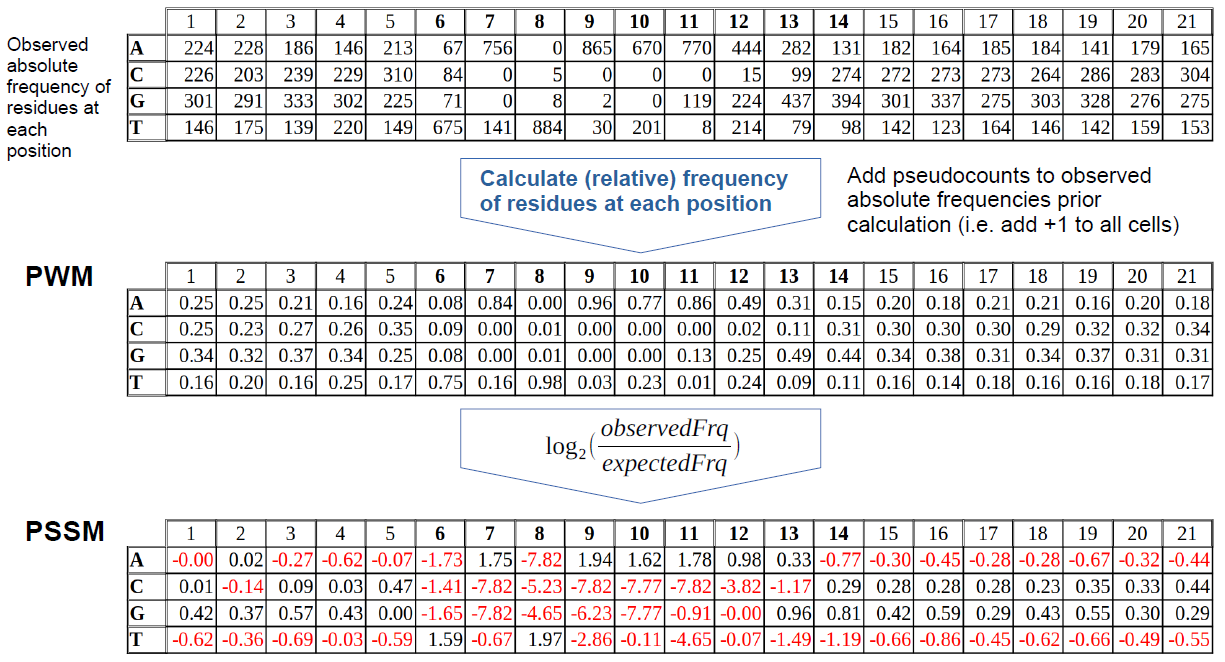
\includegraphics[width = \textwidth]{figs/tata.png}
\caption{Frecuencia de nucleótidos en el motivo TATA derivada de >800 secuencias promotoras de mamíferos de GenBank que tenían elementos TATA anotados a $\sim$ -30 pb del TSS.}
\end{figure}

\subsection{Secuencia de logotipos y contenido informativo}
Los PSSM y los HMM son formas precisas de representar la MSA. Son especialmente fáciles de manipular por ordenador y, por tanto, aptos para representar motivos y dominios proteicos en bases de datos especializadas y para buscar en bases de datos. Sin embargo, no son una forma fácil de representar MSA para el ser humano.

Por este motivo, en publicaciones y libros, los patrones de un conjunto de secuencias alineadas se suelen mostrar mediante una representación gráfica denominada \textbf{logo}. En un logo, los símbolos encontrados en cada posición del alineamiento se muestran apilados unos sobre otros, ordenados según su frecuencia (el símbolo más frecuente se muestra encima del resto). Además, la altura de los símbolos es proporcional a su frecuencia, de modo que se resaltan los símbolos preferidos en cada posición. Por último, la altura total de cada columna de símbolos se ajusta para significar la conservación global de los símbolos. Así, las posiciones que muestren una fuerte preferencia por un determinado tipo de residuos serán altas, mientras que las posiciones que muestren poca conservación estarán representadas por una pila corta de símbolos. La representación resultante revela claramente el patrón que definen las secuencias alineadas (véase la figura \ref{fig:logo}).

\begin{figure}[htbp]
\centering
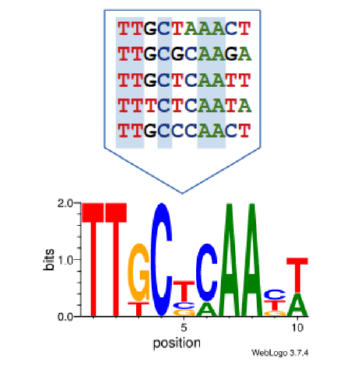
\includegraphics[width = 0.3\textwidth]{figs/logo.png}
\caption{\textbf{Logo}. Representación de la alineación mostrada en la figura \ref{fig:consensus-seq} como logo. El gráfico se generó con WebLogo3 sin ajustes de composición y utilizando un esquema de colores clásico.}
\label{fig:logo}
\end{figure}

Los logos de secuencias se basan en el concepto de entropía de la teoría de la información, desarrollado por Claude Shannon. El grado de conservación de los residuos en una posición concreta de un MSA puede cuantificarse, utilizando las herramientas de la teoría de la información, como la cantidad de incertidumbre sobre los posibles residuos que pueden ocupar esa posición. Por ejemplo, dado el MSA representado en la figura \ref{fig:logo}, nuestra incertidumbre sobre el nucleótido que puede encontrarse en la posición 1 de un sitio de unión a C/EBP es muy pequeña. Así, si alguien encuentra una nueva región unida por C/EBP será fácil predecir el nucleótido presente en la primera posición antes de ver este nuevo sitio de unión. En cambio, sería mucho más difícil predecir con certeza la identidad del residuo en la novena posición. En el campo de la información, la entropía \footnote{Formalmente, se llama entropía de Shannon}, H, de una variable aleatoria discreta X con valores posibles $x_1, x_2, \ldots ,x_n$ es una medida de la cantidad de incertidumbre asociada al valor de X (cuantifica la información). La entropía de Shannon se define como:
$$H(X) = -\sum_i P((x_i) log_2 P(x_i)$$
donde $P(x_i)$ es la probabilidad de observar el valor $i$-ésimo de X. La entropía, $H(X)$, se mide en unidades de bits. El término bit (que no byte) es una acortación de "binary digit" y representa la unidad básica de información en comunicación computacional y digital. En ese sentido, el término $P(x_i) log_2 P(x_i)$ es 0 cuando $P(x_i) = 0$.

Podemos pensar en los bits como el número mínimo de dígitos binarios necesarios para representar todos los estados de un sistema. Por ejemplo, el lanzamiento de una moneda puede dar dos resultados (estados): cara o cruz. Un solo dígito binario puede representar ambos (0 o 1). Por tanto, la entropía asociada al lanzamiento de una moneda es: $-(P_{head} log_2 P_{head} + P_{tail} log_2 P_{tail}) = 1 bit$. 
Del mismo modo, lanzar un dado puede dar lugar a 6 estados diferentes, por lo que para representar todos los casos posibles necesitaríamos tres dígitos binarios. Nótese que, en este caso, tres dígitos binarios es un exceso, ya que pueden representar hasta 8 estados (000, 001, 010, 100, 011, 101, 110, 111), mientras que nosotros sólo necesitamos representar 6. Sin embargo, dos dígitos binarios serían insuficientes para representar los seis estados. Por eso la entropía asociada es de 2,6 bits en lugar de 3. Último ejemplo: la incertidumbre de que haya un nucleótido en una cierta posición es:
\begin{align*}
H(nucleotide) = - \sum_{x_i = A, C, G, T} P(x_i) log_2 P(x_i) = \\
 - ((\frac{1}{4} \cdot log_2\frac{1}{4}) + (\frac{1}{4} \cdot log_2\frac{1}{4}) + (\frac{1}{4} \cdot log_2\frac{1}{4}) + (\frac{1}{4} \cdot log_2\frac{1}{4})) = 2 bits
\end{align*}
Por tanto, el genoma humano puede almacenar una capacidad máxima de información de:
$$3,2 \cdot 10^9 pb \cdot 2 bits = 6,4 \cdot 10^9 bits = 800 Mb = 0,8 Gb$$
Solo se tiene en cuenta una cadena y no las dos ya que, al ser complementarias, la información codificada es la misma en ambas cadenas y, por tanto, redundante. 
Bajo los estándares actuales, esta cantidad de información es ridícula. En el ADN está toda la información necesaria para hacer cualquier individuo completo. No obstante, el genoma codificante es un 1-2\%. Esto es crítico, ya que se genera mucha complejidad con tan poca información. El tema está en que nuestro genoma no codifica la información de cada neurona, solo codifica proteínas, las cuales interaccionan entre sí y generan propiedades emergentes. Así, hay una capa superpuesta de información que no es evidente y explica toda la complejidad. 
Nuestro genoma acumula muy poca información, pero es muy pequeño. Por unidad de volumen, la densidad de información a guardar es mucho más grande. Otra ventaja fundamental es que el ADN es muy estable, incluso almacenado de forma no óptima. Por ejemplo, los fósiles siguen teniendo ADN que se puede recuperar; no se puede decir lo mismo de un teléfono móvil 3 semanas a la intemperie. Por ello, se está intentando almacenar información en el ADN, pero el problema es cómo guardarlo y recuperarlo, ya que depende de procesos bioquímicos sensibles.

Volviendo a los logos, la altura de cada columna de símbolos representa el contenido informativo de esa posición concreta. Debemos pensar en el contenido informativo como una disminución de la incertidumbre tras la recepción de algún mensaje o dato. Así, el contenido informativo o entropía relativa es la diferencia entre la entropía (es decir, la incertidumbre) antes y después del mensaje:
$$I(X) = H_b(X) - H_a(X)$$
donde $I(X)$ es la información, $H_b$ la incertidumbre inicial y $H_a$ la entropía después de haber recibido algunos datos.
Por ejemplo, la incertidumbre sobre el resultado de tirar un dado antes de lanzarlo es de 2,6 bits. Si alguien tira los dados (sin que veamos el resultado) y nos informa de que el resultado ha sido un número par, entonces la entropía tras recibir este nuevo dato es de 1,6 bits. Así, podemos cuantificar la información recibida como $H_{before} - H_{after}$ correspondiente a 1 bit. En el caso de las secuencias biológicas, ver el MSA reduce nuestra incertidumbre sobre el símbolo esperado en cada posición y esta reducción se cuantifica por el contenido de información de cada posición. Nótese que hemos estado calculando el contenido de información para posiciones individuales. La ganancia total de información se obtiene sumando todas las posiciones. Al hacerlo, partimos del supuesto simplificador de que las frecuencias de una posición no se ven influidas por las de otra posición. Así, el contenido total de información para el MSA se calcula como:
$$I = \sum_i H_i^b - H_i^a$$
donde $i$ representa cada posición en el alineamiento.

\begin{table}[htbp]
\begin{mdframed}[backgroundcolor=black!10]
En resumen, los logos son representaciones de los alineamientos donde se representan los nucleótidos en cada posición, siendo el tamaño del nucleótido representativo de su frecuencia. En este caso, el eje y muestra bits, que son una unidad de información. Cuantas más posibilidades (outcome, $x_i$) hay, más incertidumbre hay y, por tanto, mayor es la entropía de Shannon. 

Algunas posiciones llegan a los 2 bits, es decir, almacenan toda la información que es posible almacenar. Sin embargo, hay otras posiciones que son menores que 2 bits. Esto se debe a que no se muestra la entropía, si no la información: la incertidumbre de un proceso antes y después de recibir información adicional. Antes de un alineamiento, la incertidumbre en cada posición es de 2 bits. Si tras hacer el alineamiento una posición tiene siempre un mismo nucleótido, la incertidumbre pasa a ser 0, por lo que la información es 2 - 0 = 2. Cuanto más variable sea una posición en el alineamiento, más incertidumbre hay y menos información tenemos. En los logos, la altura es el contenido de información y el tamaño de cada letra es la probabilidad de que salga.
\end{mdframed}
\end{table}

\begin{figure}[htbp]
\centering
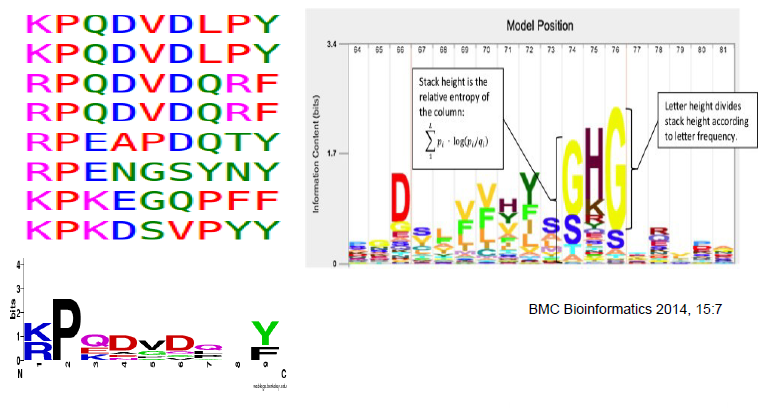
\includegraphics[width = \textwidth]{figs/logo-parts.png}
\caption{Partes de un logo.}
\end{figure}

%\subsection{Modelos de Markov ocultos (HMM)}
